% id: 0277
% book: RPM 중3-2 수학 · 03 원과 직선
% section: 유형 03 현의 수직이등분선 (3)
% figure: crop:fig-0277.png
% answer: $10\pi\mkern3mu \mathrm{cm}$
% answer_source: 답지
% variant_level: 0 (원본 전사)
% 이 파일은 build.mjs 가 items.json 에서 만든다. 고칠 때는 items.json 을 고친다.
\noindent\begin{minipage}[t]{0.58\linewidth}\vspace{0pt}\raggedright 원 모양의 접시의 깨진 일부분이 오른쪽 그림과 같을 때, 깨지기 전의 원래 접시의 둘레의 길이를 구하시오.\end{minipage}\hfill\begin{minipage}[t]{0.4\linewidth}\vspace{0pt}\centering \setlength{\dmfigw}{88.1pt}\ifdim\dmfigw>\linewidth\setlength{\dmfigw}{\linewidth}\fi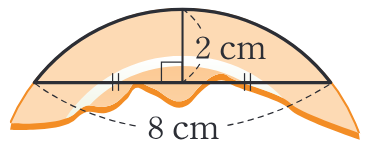
\includegraphics[width=\dmfigw]{figures/fig-0277.png}\end{minipage}\par
